\section{Konsept}
\label{sec:konsept}
\textit{En overordnet beskrivelse av \textbf{hva} systemet skal gjøre. Her legges vekt på hvordan systemet skal oppføre seg, ikke \textbf{hvordan} det er designet.}

Referer til figur!!!

Del opp i avsnitt? Litt før og litt etter figuren. 

Evt. inkluder en punktliste på hva den skal gjøre.

SKal mer inkluderes? Virker kort.

Systemet som skal designes skal overvåke fugleaktiviteten over et område. \todo{Flyttes til fremtidige forbedringer?}Flere enheter av den samme typen skal kunne kombineres for å dekke et større areal. Et infrarødt kamera skal kontinuerlig ta bilder av himmelen for å se etter varmesignaturer fra fugler. Varmesignaturen fra en fugl spores fra bilde til bilde og loggføres, og alle fugler i bildet spores individuelt. Systemet skal også innhente grunnleggende værdata: nedbør, vind, temperatur, luftfuktighet og lufttrykk. Data fra fugleaktiviteten og værforholdene skal overføres trådløst og presenteres på en nettside.

\begin{figure}[H]
    \centering
    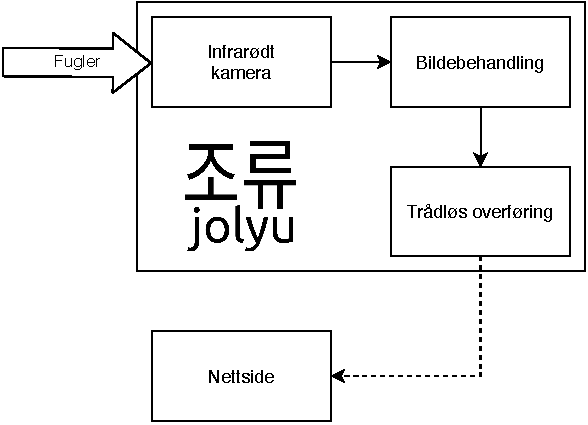
\includegraphics[width=0.75\textwidth]{konsept/Diagram_konsept.pdf}
    \caption{Blokkdiagram for konseptet.}
    \label{fig:konsept}
\end{figure}
 

$\mathbb{TEKST} \:\: \mathbb{FRA} \:\: \mathbb{INNLEVERING}$:

Systemet skal være i stand til å kunne telle fugler som flyr over et gitt område. Fuglene på himmelen skal telles og loggføres, og spores på en slik måte at en passerende fugl kun telles én gang. Dette oppnås ved at et infrarødt kamera filmer himmelen og eventuelle fuglers varmesignatur mot himmelen. Bildene analyseres i en prosesseringsenhet, som oppdager og sporer fuglene. I tillegg skal systemet inneholde sensorer for å måle værdata. Dette inkluderer nedbør, luftfuktighet, temperatur, trykk, lys, og vind. Data overføres så trådløst til en nettside, hvor den fremstilles til brukere og kan analyseres videre. Systemet kan utvides med flere kameraer for økt dekning, eller flere separate enheter. Et økt dekningsområde gir større muligheter for avansert sporing eller overvåkning av fugleaktivitet, eller for å kunne observere forskjeller i aktivitet i sanntid.




\subsection{Kamera}

Vi skal bruke et infrarødt kamera (IR-kamera) til å detektere den infrarøde strålingen fra fugler. Infrarød stråling er elektromagnetisk stråling med en bølgelengde lenger en synlig lys. (700nm-1mm). Infrarød stråling detekterer alle objekter med en temperatur over det absolutte nullpunkt (0K) og opp til 3864K. Vi er mest interessert i temperaturer rundt kroppstemperaturen til fugler (40 K https://www.sciencedirect.com/science/article/pii/030096299190122S) sett i forhold til omgivelsene fra -15 til 30 C sett i forhold til maks og minimumstemperaturer i trondheim det siste året. Dette tilsvarer bølgelenden i langbølge IR på $8-15\mu m$. Et IR-kamera bruker Stephen-Boltzmanns lov for å regne ut temperaturen til objektet $R=\epsilon \sigma T^2$ der R er infrarød stråling (W/$m^2$), T er temperatur i kelvin, $\sigma$ er boltzmanns konstant og $\epsilon$ er den termiske emissiviteten til objektet som skal måles. For fugler er denne emissiviteten målt til å være ca 0.95 (Temperature Biology
of Animals, cossin bowler 1987). 


Vi bruker et infrarødt kamera som ser etter varmesignaturen til fugler. hovedsensor for detektering av fugler. Kameraet skal gi prosseseringsenheten en kontinuerlig sendig av video.


\subsection{Deteksjon}
Systemet skal kunne detektere fugler fra en kontinuerlig videostrømm. Fuglene skal 



\subsection{Nettside}


